% figures/fig2_boltzmann.tex -- float wrapper for Figure 2 (cited from Sec. 5.2).
% Image produced by figures/make_experiment_figures.py --only fig2.
% P-F1 RETIRED 2026-08-03: figures/dump_boltz_records.py was run over the n=120
% arms, so <tag>/boltz_records.csv now exists and the three left panels plot the
% measured (log q_theta, -E_xTB/kT) pairs.  The script reports mode=records.
\begin{figure}[t]
\begin{center}
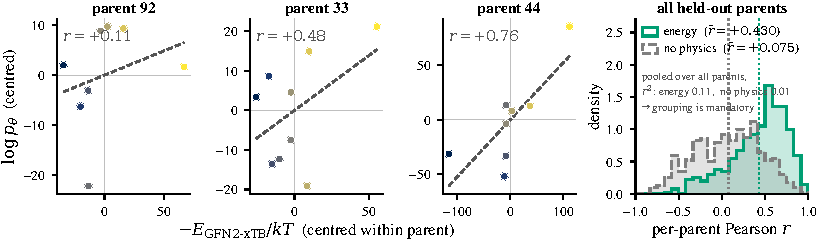
\includegraphics[width=\linewidth]{figures/out/fig2_boltzmann_scatter.pdf}
\end{center}
\caption{The model's log-density \emph{orders} geometries by energy within each parent; the scale
read-out of the same models is \Cref{tab:scale}, and it does not improve.
Left three panels: three parents at the 20th, 55th and 92nd percentile of the measured
per-parent Pearson $r$, so the panels span the observed spread rather than only its successes;
each point is one evaluation geometry with its measured $\log q_\theta$ and its GFN2-xTB
energy, both axes centred within the parent, and the dashed line is the per-parent
least-squares fit. Right: the distribution of $r_m$ over all 120 held-out parents for the
energy-supervised model and for the no-physics flow-matching control, with dotted lines at the
means ($+0.434$ and $+0.074$; this panel plots the permissive, reference-included metric over all
120 parents, not the primary endpoint of column 1 of \Cref{tab:boltzmann}). Pooling all parents into a single regression destroys the signal
($r^2 = 0.11$ and $0.01$), because between-molecule free-energy offsets dominate the pooled
variance; this is why the metric is defined within parents.}
\label{fig:boltzmann}
\end{figure}
